\section{Manifold Mixup}
\label{sec:manifoldmixup}

Manifold mixup trains neural networks on linear combinations of hidden representations of training examples~\cite{verma19}.
Hence, it performs mixup in an intermediate layer in which feature spaces are more aligned.
Furthermore, a neural network trained with manifold mixup learns class-representations with fewer directions of variance and yields a smoother decision boundary.

Training a deep neural network using manifold mixup is done as follows:
We select a layer $k$ at random from the set of eligible layers $\mathcal{S}$ in the neural network. 
$\mathcal{S}$ may contain the first layers of the residual blocks, for instance.
Then perform input mixup~\cite{zhang17} on two random minibatches $(x_i, y_i)$ and $(x_j,y_j)$ which are processed through the forward pass until reaching layer $k$. This gives us a mixed minibatch $(\tilde{x}, \tilde{y})$.
With that we continue the forward pass from layer $k$ until we ultimately get the output.
Finally, we update the parameters of the neural network by computing the loss and gradients using the output.

\subsection{Implementation}

Manifold mixup can be implemented in a few lines of code without heavy computations that would drop the training performance of the deep neural network a lot.

\begin{code}{Mixup implementation}{lst:mixup}
def mixup(x, y, alpha):
    batch_size = x.size()[0]
    lam = np.random.beta(alpha, alpha) if mixup_alpha > 0 else 1

    if torch.cuda.is_available():
        index = torch.randperm(batch_size).cuda()
    else:
        index = torch.randperm(batch_size)

    # x[index, :] swaps the training samples
    mixed_x = lam * x + (1 - lam) * x[index, :]
    y_a, y_b = y, y[index]
    
    return mixed_x, y_a, y_b
\end{code}

Listing~\ref{lst:mixup} shows the actual mixup procedure that 
(1) draws $\lambda$ from the Beta distribution (line 3),
(2) picks batch-size many random indices (line 6 and 8, respectively),
(3) mixes each sample in the batch with another sample determined by the random indices (line 11).

\newpage
\subsection{Visualization}

Figure~\ref{fig:visualization} visualizes three examples of the mixup process using $\lambda = 0.5$.

\begin{figure}[ht]
    \centering
    \begin{minipage}{.25\columnwidth}
        \centering
        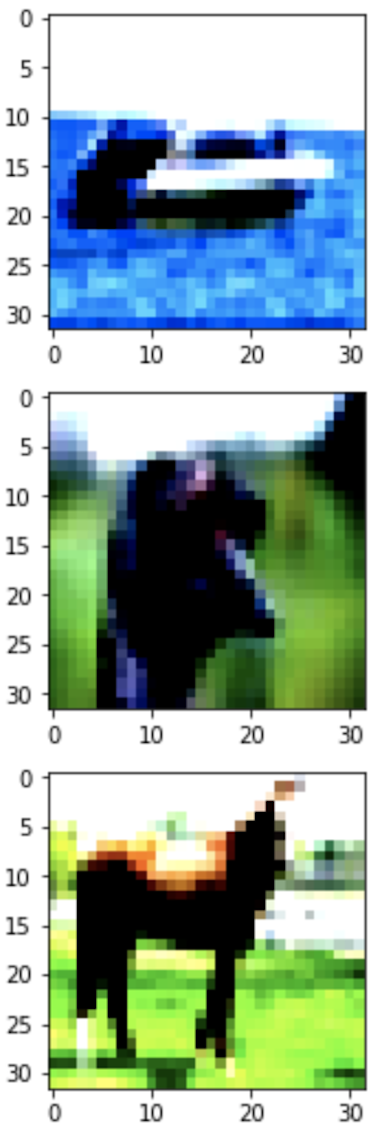
\includegraphics[width=0.7\textwidth]{figures/1.png} \\
        (a)
    \end{minipage}
    \begin{minipage}{.25\columnwidth}
        \centering
        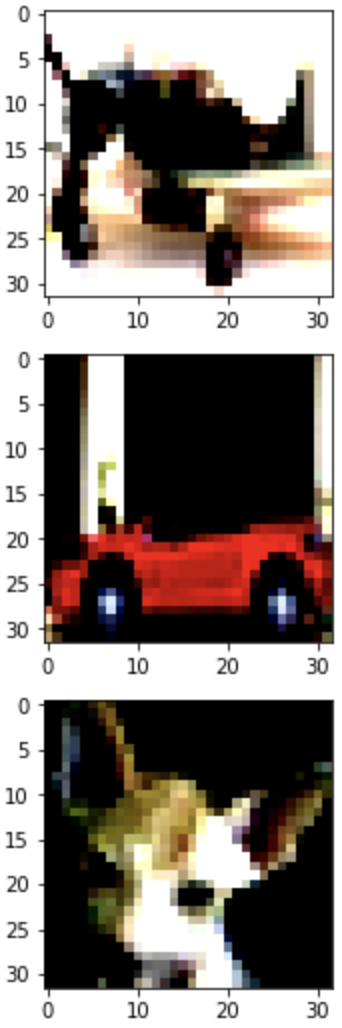
\includegraphics[width=0.7\textwidth]{figures/2.png} \\
        (b)
    \end{minipage}
    \begin{minipage}{.25\columnwidth}
        \centering
        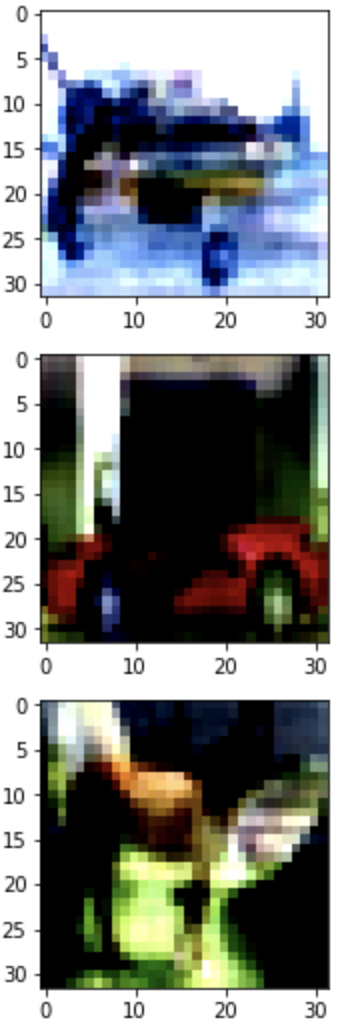
\includegraphics[width=0.7\textwidth]{figures/3.png} \\
        (c)
    \end{minipage}

    \caption{Mixup visualized: (a) and (b) depict two randomly drawn samples, respectively, (c) the mixup outcome of (a) and (b) by setting $\lambda$ to $0.5$. Each row represents a different example.}
    \label{fig:visualization}
\end{figure}